\icode{N17SU-ME-CA-L3-260625-001}
\nceeID[16]{2017江苏}{22}
如图所示，两个半圆柱\(A\)、\(B\)紧靠着静置于水平地面上，其上有一光滑圆柱\(C\)，三者半径均为\(R\)。\(C\)的质量为\(m\)，\(A\)、\(B\)的质量都为\(\frac{m}{2}\)，与地面的动摩擦因数均为\(\mu\)。现用水平向右的力拉\(A\)，使\(A\)缓慢移动，直至\(C\)恰好降到地面。整个过程中\(B\)保持静止。设最大静摩擦力等于滑动摩擦力，重力加速度为\(g\)。求：
\begin{enumerate}[(1)]
	\item 未拉\(A\)时，\(C\)受到\(B\)作用力的大小\(F\)；
	\item 动摩擦因数的最小值\(\mu_{\mathrm{min}}\)；
	\item \(A\)移动的整个过程中，拉力做的功\(W\)。
\end{enumerate}
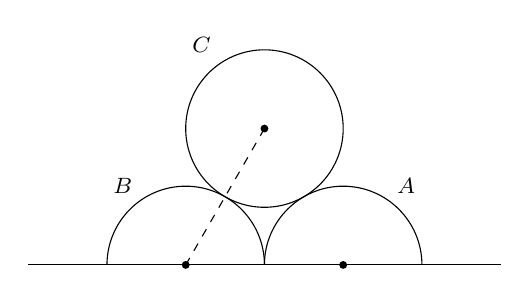
\begin{tikzpicture}[font=\footnotesize]
	\draw (0,0) arc(0:180:1);
	\draw (2,0) arc(0:180:1);
	\draw (0,{sqrt(3)})circle(1);
	\draw (-3,0)--(3,0);
	\draw[dashed] (0,{sqrt(3)})--(-1,0);
	\fill (-1,0) circle(.05);
	\fill (1,0) circle(.05);
	\fill (0,{sqrt(3)}) circle(.05);
	\node at(-1.8,1){\(B\)};
	\node at(1.8,1){\(A\)};
	\node at(-.8,2.8){\(C\)};
\end{tikzpicture}